\documentclass[11pt]{article}


%%% Packages
%%
\usepackage{amsmath}
\usepackage{amsfonts}
\usepackage{amssymb}
\usepackage{fancyhdr}
\usepackage{float}
\usepackage{graphicx}
\usepackage{listings}
\usepackage{enumitem}
\usepackage[margin = 1in, headheight = 13.6pt]{geometry}
\usepackage[linktoc=all]{hyperref}
%%
%%%


%%% Formatting
%%
\parindent 0em
\parskip 1em
\pagestyle{fancy}
\fancyhead{}
\fancyfoot{}
\fancyhead[L]{\slshape\MakeUppercase{{\myTitle}}}
\fancyhead[R]{\slshape{\myName}}
\fancyfoot[C]{\thepage}
%%
%%%


%%% User defined variables
%%
\def \myTitle {ECE 302 Homework 4}
\def \myName {Elias Talcott}
\def \myDate {October 12, 2020}
%%
%%%


\begin{document}

\section{Exercise 8 Python Code}
\lstinputlisting[language=Python, breaklines=True]{exercise8.py}

\pagebreak

\section{Exercise 8 Result}
\begin{figure}[h!]
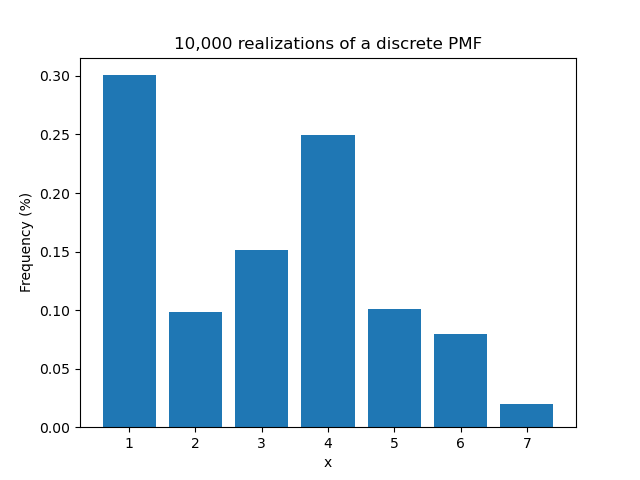
\includegraphics[width=0.8\linewidth]{histogram.png}
\end{figure}


\end{document}